\documentclass[11pt,a4paper,oneside]{report}

% ------------------------------------------------------------
% Encoding, typography, and page geometry
% ------------------------------------------------------------
\usepackage[T1]{fontenc}
\usepackage[utf8]{inputenc}
\usepackage{lmodern}
\usepackage{microtype}
\usepackage[
    a4paper,
    left=2.4cm,
    right=2.4cm,
    top=2.3cm,
    bottom=2.5cm,
    headheight=40pt,
    headsep=0.65cm,
    footskip=1.05cm
]{geometry}

% ------------------------------------------------------------
% Mathematics
% ------------------------------------------------------------
\usepackage{amsmath}
\usepackage{amssymb}
\usepackage{mathtools}

% ------------------------------------------------------------
% Tables and lists
% ------------------------------------------------------------
\usepackage{booktabs}
\usepackage{tabularx}
\usepackage{array}
\usepackage{longtable}
\usepackage{multirow}
\usepackage{enumitem}
\usepackage{multicol}
\newcolumntype{P}[1]{>{\raggedright\arraybackslash}p{#1}}

% ------------------------------------------------------------
% Colour and semantic boxes
% ------------------------------------------------------------
\usepackage[table]{xcolor}
\usepackage[most]{tcolorbox}

\definecolor{SapienzaRed}{RGB}{148,28,50}
\definecolor{SapienzaRedDark}{RGB}{112,20,37}
\definecolor{SapienzaRedPale}{RGB}{250,242,244}
\definecolor{KeyGreen}{RGB}{43,87,61}
\definecolor{KeyGreenPale}{RGB}{242,248,244}
\definecolor{NeutralGray}{RGB}{80,80,80}
\definecolor{NeutralGrayPale}{RGB}{247,247,247}
\definecolor{PlotBlue}{RGB}{57,88,119}
\definecolor{DarkText}{RGB}{30,30,30}
\colorlet{SoftRed}{SapienzaRedPale}
\colorlet{SoftBlue}{SapienzaRedPale}
\colorlet{SoftGreen}{KeyGreenPale}
\colorlet{SoftGray}{NeutralGrayPale}
\colorlet{MidGray}{NeutralGray}

\newtcolorbox{definitionbox}[1][]{
    enhanced,
    breakable,
    colback=SapienzaRedPale,
    colframe=SapienzaRed,
    colbacktitle=SapienzaRed,
    coltitle=white,
    fonttitle=\bfseries,
    title={Definition#1},
    boxrule=0.65pt,
    arc=1.4mm,
    left=2.5mm,right=2.5mm,top=1.6mm,bottom=1.6mm
}

\newtcolorbox{keyconcept}{
    enhanced,
    breakable,
    colback=KeyGreenPale,
    colframe=KeyGreen,
    colbacktitle=KeyGreen,
    coltitle=white,
    fonttitle=\bfseries,
    title={Key Concept},
    boxrule=0.65pt,
    arc=1.4mm,
    left=2.5mm,right=2.5mm,top=1.6mm,bottom=1.6mm
}

\newtcolorbox{remarkbox}[1][]{
    enhanced,
    breakable,
    colback=NeutralGrayPale,
    colframe=NeutralGray,
    colbacktitle=NeutralGray,
    coltitle=white,
    fonttitle=\bfseries,
    title={Remark#1},
    boxrule=0.55pt,
    arc=1.4mm,
    left=2.5mm,right=2.5mm,top=1.6mm,bottom=1.6mm
}

\newtcolorbox{examplebox}[1][]{
    enhanced,
    breakable,
    colback=SapienzaRedPale,
    colframe=SapienzaRedDark,
    colbacktitle=SapienzaRedDark,
    coltitle=white,
    fonttitle=\bfseries,
    title={Example#1},
    boxrule=0.6pt,
    arc=1.4mm,
    left=2.5mm,right=2.5mm,top=1.6mm,bottom=1.6mm
}

\newtcolorbox{metricbox}[1][]{
    enhanced,
    colback=white,
    colframe=SapienzaRed,
    colbacktitle=SapienzaRed,
    coltitle=white,
    fonttitle=\bfseries,
    title={Performance Metric#1},
    boxrule=0.75pt,
    arc=1.4mm,
    left=2.5mm,right=2.5mm,top=1.6mm,bottom=1.6mm
}

% ------------------------------------------------------------
% Figures, plots, and code
% ------------------------------------------------------------
\usepackage{graphicx}
\usepackage{float}
\usepackage{tikz}
\newif\ifTikZAvailable
\TikZAvailabletrue
\usetikzlibrary{
    arrows.meta,
    positioning,
    fit,
    calc,
    shapes.geometric,
    backgrounds
}
\usepackage{pgfplots}
\pgfplotsset{compat=1.18}
\usepackage{listings}
\lstset{
    basicstyle=\ttfamily\small,
    frame=single,
    rulecolor=\color{NeutralGray},
    backgroundcolor=\color{NeutralGrayPale},
    breaklines=true,
    columns=fullflexible,
    showstringspaces=false
}

% ------------------------------------------------------------
% Captions, headings, references, and page style
% ------------------------------------------------------------
\usepackage{caption}
\captionsetup{
    font=small,
    labelfont=bf,
    textfont=normalfont
}

\usepackage{needspace}
\usepackage{fancyhdr}
\usepackage{titlesec}
\usepackage{hyperref}

\hypersetup{
    colorlinks=true,
    linkcolor=SapienzaRed,
    citecolor=SapienzaRed,
    urlcolor=SapienzaRedDark,
    pdftitle={Biometric Systems - Lecture Notes},
    pdfauthor={Matt Clifford Trinidad Ramos}
}

\titleformat{\chapter}[hang]
    {\normalfont\huge\bfseries\color{DarkText}\raggedright\hyphenpenalty=10000\exhyphenpenalty=10000}
    {\color{SapienzaRed}\thechapter}
    {0.7em}
    {}
\titlespacing*{\chapter}{0pt}{-8pt}{22pt}

\titleformat{\section}
    {\normalfont\Large\bfseries\color{DarkText}}
    {\color{SapienzaRed}\thesection}
    {0.6em}
    {}
\titlespacing*{\section}{0pt}{2.0ex plus .4ex}{0.8ex}

\titleformat{\subsection}
    {\normalfont\large\bfseries\color{DarkText}}
    {\color{SapienzaRed}\thesubsection}
    {0.55em}
    {}

\setcounter{tocdepth}{2}
\setcounter{secnumdepth}{2}

\pagestyle{fancy}
\fancyhf{}
\newcommand{\CurrentSectionMark}{}
\renewcommand{\chaptermark}[1]{%
    \gdef\CurrentSectionMark{}%
    \markboth{\thechapter\quad #1}{}%
}
\makeatletter
\renewcommand{\sectionmark}[1]{%
    \protected@xdef\CurrentSectionMark{\thesection\quad\unexpanded{#1}}%
    \markright{\CurrentSectionMark}%
}
\makeatother
% Re-emit the active section mark at the start of each paragraph.  This makes
% the right-hand header describe the section that is actually active at the
% top of a continuation page instead of a later section that happens to begin
% farther down on the same page.
\AddToHook{para/begin}{%
    \ifx\CurrentSectionMark\empty\else
        \markright{\CurrentSectionMark}%
    \fi
}
\fancyhead[L]{\parbox[b]{0.48\headwidth}{\small\raggedright\nouppercase{\leftmark}}}
\fancyhead[R]{\parbox[b]{0.48\headwidth}{\small\raggedleft\nouppercase{\rightmark}}}
\fancyfoot[L]{\scriptsize BIOMETRIC SYSTEMS}
\fancyfoot[C]{\small\thepage}
\fancyfoot[R]{\scriptsize Matt Clifford Trinidad Ramos}
\renewcommand{\headrulewidth}{0.45pt}
\renewcommand{\footrulewidth}{0.35pt}
\makeatletter
\renewcommand{\headrule}{%
  \hbox to\headwidth{\color{SapienzaRed}\leaders\hrule height \headrulewidth\hfill}}
\renewcommand{\footrule}{%
  \hbox to\headwidth{\color{SapienzaRed}\leaders\hrule height \footrulewidth\hfill}}
\makeatother

\fancypagestyle{plain}{
    \fancyhf{}
    \fancyfoot[L]{\scriptsize BIOMETRIC SYSTEMS}
    \fancyfoot[C]{\small\thepage}
    \fancyfoot[R]{\scriptsize Matt Clifford Trinidad Ramos}
    \renewcommand{\headrulewidth}{0pt}
    \renewcommand{\footrulewidth}{0.35pt}
}

% ------------------------------------------------------------
% Paragraph and float behaviour
% ------------------------------------------------------------
\setlength{\parindent}{1.15em}
\setlength{\parskip}{0.18em}
\setlength{\emergencystretch}{2.5em}
\clubpenalty=4000
\widowpenalty=4000
\displaywidowpenalty=4000
\raggedbottom
\renewcommand{\arraystretch}{1.18}
\setlength{\tabcolsep}{5pt}
\setlist[itemize]{topsep=0.45em,itemsep=0.15em}
\setlist[enumerate]{topsep=0.45em,itemsep=0.2em}

% ------------------------------------------------------------
% Mathematical notation
% ------------------------------------------------------------
\newcommand{\R}{\mathbb{R}}
\newcommand{\Prob}{\Pr}
\newcommand{\E}{\mathbb{E}}
\newcommand{\norm}[1]{\left\lVert #1 \right\rVert}
\newcommand{\set}[1]{\left\{ #1 \right\}}
\newcommand{\abs}[1]{\left| #1 \right|}
\newcommand{\id}{\operatorname{id}}
\newcommand{\topMatch}{\operatorname{topMatch}}
\newcommand{\rankop}{\operatorname{rank}}

\begin{document}
\hypersetup{pageanchor=false}

% ============================================================
% Title page
% ============================================================
\begin{titlepage}
    \thispagestyle{empty}
    \centering

    \vspace*{1.05cm}

    % Official logo from Sapienza's downloadable visual identity assets.
    
\includegraphics[
        width=0.52\textwidth,
        keepaspectratio
    ]{sapienza_logo.png}\par

    \vspace{1.15cm}

    {\color{SapienzaRed}\rule{0.82\textwidth}{0.9pt}\par}

    \vspace{0.75cm}

    {\LARGE\bfseries\MakeUppercase{BIOMETRIC SYSTEMS}\par}

    \vspace{0.35cm}

    {\Large Lecture Notes\par}

    \vspace{0.75cm}

    {\color{SapienzaRed}\rule{0.82\textwidth}{0.9pt}\par}

    \vfill

    {\small\textsc{Lecturer}\par}
    \vspace{0.12cm}
    {\large Maria De Marsico\par}

    \vspace{0.8cm}

    {\small Department of Computer Science\par}
    {\small Sapienza University of Rome\par}

    \vspace{1.3cm}

    {\small\textsc{Notes prepared by}\par}
    \vspace{0.12cm}
    {\large\bfseries Matt Clifford Trinidad Ramos\par}

    \vfill
\end{titlepage}
\hypersetup{pageanchor=true}

\pagenumbering{roman}
\tableofcontents
\clearpage

\pagenumbering{arabic}
\pagestyle{fancy}

\chapter{Introduction to Biometric Systems}
\label{sec:introduction}

Biometric recognition identifies or authenticates people from measurable
physical or behavioural characteristics. The central engineering problem is
to transform variable sensor observations into representations that remain
discriminative across people and sufficiently stable for repeated use.

% ============================================================

\section{Biometrics as Pattern Recognition}
\label{subsec:pattern-recognition}

A biometric system can be understood as a particular form of
\emph{pattern-recognition system}. A sample acquired from a person is
represented through a collection of measurable characteristics, often
summarized by a feature vector.

Two patterns are considered similar when an appropriate distance between
their feature representations is sufficiently small, or equivalently
when a similarity score is sufficiently large.

Three design questions determine whether a pattern-recognition pipeline can support reliable biometric matching:

\begin{enumerate}
    \item Which distance or similarity measure is appropriate?

    \item Which features are sufficiently informative and discriminative?

    \item Which difference margin, or acceptance threshold, should be used
    to decide whether two patterns match?
\end{enumerate}

Pattern recognition appears in different forms depending on the meaning
of the classes.

In content-based image retrieval, classes can correspond to different
object types, so the pattern representation separates, for example,
a face from a flower.

In a more specific recognition problem, classes may correspond to
subclasses of the same general type.

In biometrics, the classes are the \emph{individuals themselves}:
the pattern must distinguish one person from another.

\begin{keyconcept}
Biometrics uses pattern-recognition techniques in a setting where the
identities of individual people are the classes to be discriminated.
\end{keyconcept}

\section{What Is Biometrics?}
\label{subsec:what-biometrics}

The term \emph{biometrics} derives from the Greek words
\emph{bios} (life) and \emph{m\'etron} (measure).

In a broad sense, it refers to the measurement and statistical analysis
of biological data.

In technological applications, biometrics concerns the
measurement and analysis of physical and/or behavioural characteristics
for recognizing or authenticating a person.

\begin{definitionbox}[ -- Biometrics]
Biometrics is the automatic recognition of a person according to
discriminative characteristics. In operational systems, measurable
physical or behavioural traits are acquired, represented, compared,
and used to support an identity decision.
\end{definitionbox}

The basic assumption is that each person is unique.

Turning this assumption into a working system requires three main steps:

\begin{itemize}
    \item determine features that are sufficiently distinctive to identify
    a person;

    \item find reliable techniques for measuring those features;

    \item design reliable algorithms that can recognize or classify a
    person from the measured features.
\end{itemize}

\section{Access Types}
\label{subsec:access-types}

Biometric recognition can protect both physical and logical resources.

\begin{table}[htbp]
\centering
\caption{Access types considered in biometric applications.}
\label{tab:access-types}
\small

\begin{tabular}{>{\bfseries}P{3.2cm} P{10.1cm}}
\toprule
\rowcolor{SoftRed}
Access type & \textbf{Examples} \\
\midrule
Physical access & Room, building, controlled area. \\
Logical access & Electronic resources, critical data. \\
\bottomrule
\end{tabular}
\end{table}

\section{Why Biometric Systems?}
\label{subsec:why-biometrics}

Traditional authentication commonly relies on two factors.

The first is \emph{something one owns}, such as a card or document.

Such an object can be lost, stolen, or copied, and the system may
effectively authenticate the object rather than the legitimate owner.

The second is \emph{something one knows}, such as a password.

A password may be guessed, elicited from the user, or forgotten.

Moreover, a password that is easy to remember can also be easier to guess.

Biometric recognition adds a third possibility:
\emph{something one is}.

The identity evidence is derived from the person's own physical or
behavioural characteristics.

\begin{table}[htbp]
\centering
\caption{Authentication factors used in biometric authentication.}
\label{tab:auth-factors}
\small

\begin{tabular}{>{\bfseries}P{3.25cm} P{2.7cm} P{8.1cm}}
\toprule
\rowcolor{SoftRed}
Factor & \textbf{Example} &
\textbf{Main limitation} \\
\midrule

Something one owns &
Card, document &
Can be lost, stolen, or copied; the object rather than its owner may be
authenticated. \\

Something one knows &
Password &
Can be guessed, extracted from the user, or forgotten. \\

Something one is &
Biometric trait &
Recognition is based on measurable characteristics of the person;
accuracy and trait-specific limitations remain. \\

\bottomrule
\end{tabular}
\end{table}


\section{Historical Background}
\label{subsec:history}

Biometric recognition predates digital sensors and machine learning. Early
identification systems already pursued the same two properties that remain
central today: measurements should distinguish different people and should
remain sufficiently stable over time.

\subsection{Bertillon and Bertillonage}

In 1882, Alphonse Bertillon (1853--1914), chief of the identification
service of the Paris police, introduced an anthropometric identification
procedure later known as \emph{Bertillonage}. The method recorded bodily
measurements and descriptive characteristics such as hand shape, bust and
limb measurements, head shape, facial details, and the corresponding
identification card.

The method was not based on one measurement alone. Measurements were divided
into discrete categories so that records could first be partitioned into
smaller groups and only then compared in detail. The historical scheme
described \(243\) primary categories; further subdivision using seven eye
categories together with hair colour produced \(1{,}701\) groupings. With a
collection of \(5{,}000\) records, a primary category would contain roughly
\(20\) cards, reducing a search from the whole archive to a small candidate set.

\begin{examplebox}[ -- The Will West case]
In 1903, a newly admitted prisoner named Will West was measured using the
Bertillon procedure. The resulting measurements led to an existing record
for William West, whose measurements and appearance were strikingly similar.
Further investigation established that William West was already incarcerated
and that the two men were different individuals. The case illustrates the
central limitation of coarse anthropometric categorization: two people can
fall into nearly the same measurement classes even when their identities are
different.
\end{examplebox}

The rapid growth of early identification archives also made indexing an
engineering concern. Anthropometry was introduced into a United States prison
setting in 1887 by Major McClaughry. A National Bureau of Identification was
established in 1896 and was described as a forerunner of later federal
identification services. The historical account reports \(16{,}000\) Bertillon
cards after one year, \(24{,}000\) after two years, and \(131\) prisoners recorded
as first offenders who were found to have prior records. By 1900, the prison
administration was formally permitted to accept Bertillon cards.

\begin{remarkbox}[ -- Historical context]
Bertillonage is important as an early model of biometric identification, not
as a modern biometric specification. Its lasting contribution is the attempt
to formalize human identification through measurable, persistent, and
discriminative characteristics.
\end{remarkbox}

\subsection{Galton and Fingerprints}

At the end of the nineteenth century, Francis Galton criticized
anthropometric identification from a statistical point of view. In 1892 he
introduced the notion of a fingerprint \emph{minutia} and proposed an early
fingerprint classification method.

In 1893, the UK Home Office recognized the individuality of fingerprints.
Police organizations subsequently began acquiring and storing fingerprint
records and developing systematic methods for visual comparison. Around 1900,
the Galton--Henry classification system became an important basis for
fingerprint-recognition practice in many police organizations.

\section{Limitations and Integration with Traditional Systems}
\label{subsec:integration}

Biometric recognition does not always work perfectly.

Recognition failures motivate integration with traditional authentication factors.

Combining different forms of evidence can increase the security level
compared with relying on only one factor.

\begin{figure}[htbp]
\centering

\ifTikZAvailable

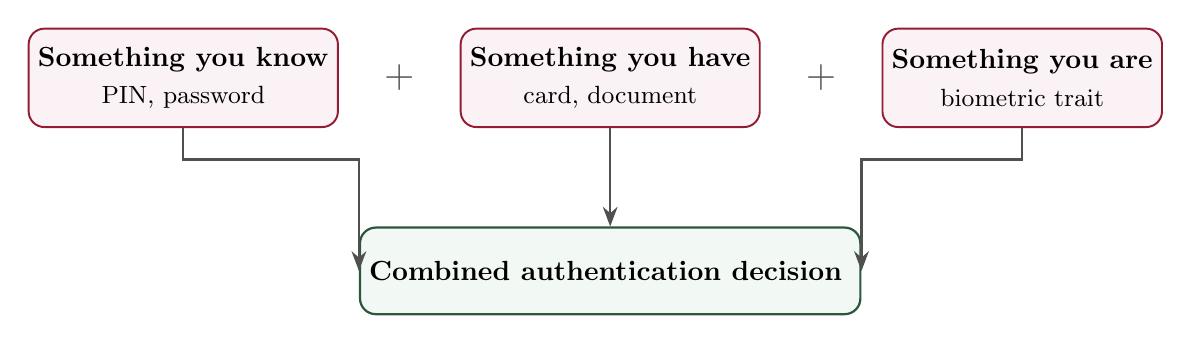
\begin{tikzpicture}[
    node distance=0.55cm,
    factor/.style={
        draw=SapienzaRed,
        rounded corners=2mm,
        fill=SoftRed,
        minimum width=3.5cm,
        minimum height=1.25cm,
        align=center,
        line width=0.7pt
    },
    decision/.style={
        draw=KeyGreen,
        rounded corners=2mm,
        fill=SoftGreen,
        minimum width=5.0cm,
        minimum height=1.1cm,
        align=center,
        line width=0.8pt
    },
    plus/.style={
        font=\Large\bfseries,
        text=MidGray
    },
    arrow/.style={
        -{Stealth[length=2.5mm]},
        line width=0.8pt,
        color=MidGray
    }
]
%
\node[factor] (know) {
    \textbf{Something you know}\\[0.15em]
    \small PIN, password
};
%
\node[plus, right=0.45cm of know] (p1) {$+$};
%
\node[factor, right=0.45cm of p1] (have) {
    \textbf{Something you have}\\[0.15em]
    \small card, document
};
%
\node[plus, right=0.45cm of have] (p2) {$+$};
%
\node[factor, right=0.45cm of p2] (are) {
    \textbf{Something you are}\\[0.15em]
    \small biometric trait
};
%
\node[
    decision,
    below=1.25cm of have
] (decision) {
    \textbf{Combined authentication decision}
};
%
\draw[arrow]
    (know.south)
    --
    ++(0,-0.40)
    -|
    (decision.west);
%
\draw[arrow]
    (have.south)
    --
    (decision.north);
%
\draw[arrow]
    (are.south)
    --
    ++(0,-0.40)
    -|
    (decision.east);
%
\end{tikzpicture}

\else

\fbox{
\begin{minipage}{0.90\textwidth}
\centering

\textbf{Something you know}
(PIN/password)

\quad+\quad

\textbf{Something you have}
(card/document)

\quad+\quad

\textbf{Something you are}
(biometric trait)
\[
\Downarrow
\]

\textbf{Combined authentication decision}

\end{minipage}
}

\fi

\caption{Combination of knowledge, possession, and biometric evidence.}
\label{fig:multifactor}

\end{figure}

Figure~\ref{fig:multifactor} summarizes the three forms of authentication
evidence discussed above.

\section{Architecture of a Biometric System}
\label{subsec:architecture}

A biometric system operates in two conceptually distinct phases:
\emph{enrollment} and \emph{recognition}.

During enrollment, biometric data are captured and processed so that a
reference template can be stored for future operations.

During recognition, newly acquired biometric data are converted into a
probe template and compared with stored templates to support a decision.

\begin{definitionbox}[ -- Enrollment]
Enrollment is the capture and processing of a user's biometric data for
use by the system in subsequent authentication or recognition operations.
The resulting reference templates populate the gallery.
\end{definitionbox}

\begin{definitionbox}[ -- Recognition]
Recognition is the capture and processing of biometric data in order to
produce an authentication or identity decision from the result of matching
a current template against stored template information.
\end{definitionbox}

\begin{definitionbox}[ -- Probe and Gallery]
A \emph{probe} is a template submitted to the system for recognition.
The \emph{gallery} is the set of templates associated with enrolled
subjects.
\end{definitionbox}

\begin{figure}[htbp]
\centering

\ifTikZAvailable

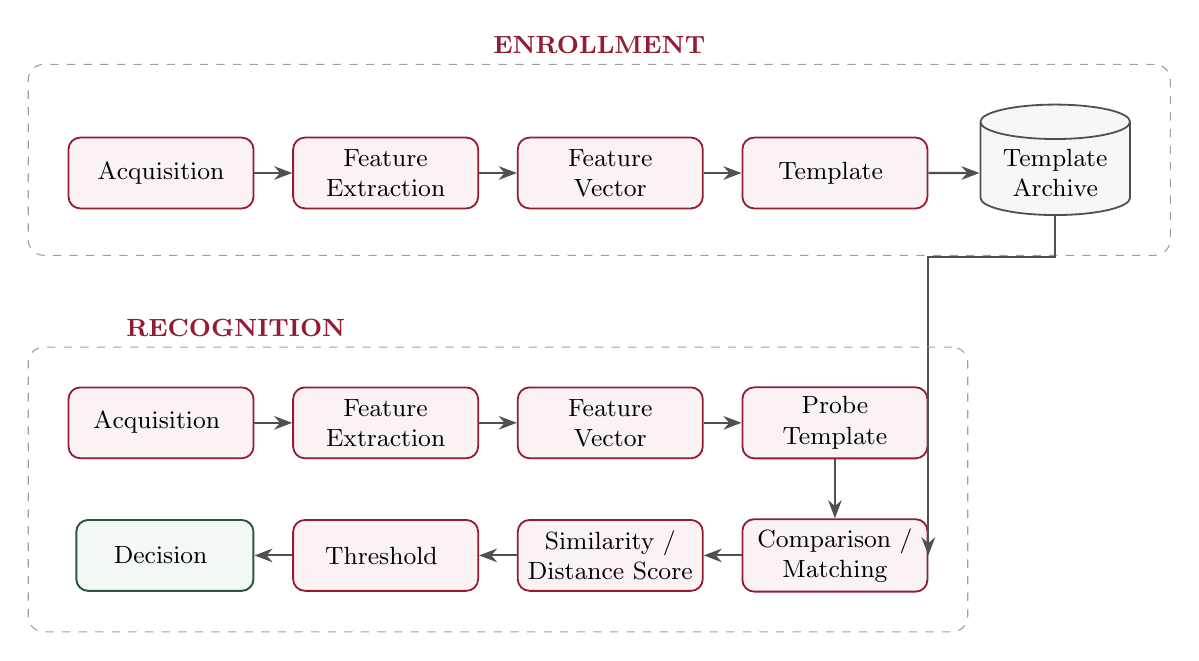
\begin{tikzpicture}[
    node distance=0.48cm and 0.48cm,
%
    process/.style={
        draw=SapienzaRed,
        rounded corners=1.5mm,
        fill=SoftBlue,
        minimum width=2.35cm,
        minimum height=0.9cm,
        align=center,
        font=\small,
        line width=0.65pt
    },
%
    archive/.style={
        draw=MidGray,
        cylinder,
        shape border rotate=90,
        aspect=0.28,
        fill=SoftGray,
        minimum width=1.9cm,
        minimum height=1.35cm,
        align=center,
        font=\small,
        line width=0.65pt
    },
%
    decision/.style={
        draw=KeyGreen,
        rounded corners=1.5mm,
        fill=SoftGreen,
        minimum width=2.25cm,
        minimum height=0.9cm,
        align=center,
        font=\small,
        line width=0.7pt
    },
%
    arrow/.style={
        -{Stealth[length=2.3mm]},
        line width=0.75pt,
        color=MidGray
    },
%
    group/.style={
        draw=MidGray!55,
        dashed,
        rounded corners=2mm,
        inner sep=5mm
    }
]
%
% Enrollment row
%
\node[process] (eacq) {Acquisition};
%
\node[
    process,
    right=of eacq
] (efeat) {
    Feature\\
    Extraction
};
%
\node[
    process,
    right=of efeat
] (evec) {
    Feature\\
    Vector
};
%
\node[
    process,
    right=of evec
] (etemp) {
    Template
};
%
\node[
    archive,
    right=0.65cm of etemp
] (archive) {
    Template\\
    Archive
};
%
\draw[arrow] (eacq) -- (efeat);
\draw[arrow] (efeat) -- (evec);
\draw[arrow] (evec) -- (etemp);
\draw[arrow] (etemp) -- (archive);
%
\node[
    group,
    fit=(eacq)(archive),
    label={
        [font=\bfseries\small,text=SapienzaRed]
        above:ENROLLMENT
    }
] (egroup) {};
%
% Recognition first row
%
\node[
    process,
    below=2.25cm of eacq
] (racq) {
    Acquisition
};
%
\node[
    process,
    right=of racq
] (rfeat) {
    Feature\\
    Extraction
};
%
\node[
    process,
    right=of rfeat
] (rvec) {
    Feature\\
    Vector
};
%
\node[
    process,
    right=of rvec
] (rprobe) {
    Probe\\
    Template
};
%
% Recognition second row
%
\node[
    process,
    below=0.75cm of rprobe
] (match) {
    Comparison /\\
    Matching
};
%
\node[
    process,
    left=of match
] (score) {
    Similarity /\\
    Distance Score
};
%
\node[
    process,
    left=of score
] (threshold) {
    Threshold
};
%
\node[
    decision,
    left=of threshold
] (rdecision) {
    Decision
};
%
\draw[arrow] (racq) -- (rfeat);
\draw[arrow] (rfeat) -- (rvec);
\draw[arrow] (rvec) -- (rprobe);
\draw[arrow] (rprobe) -- (match);
\draw[arrow] (match) -- (score);
\draw[arrow] (score) -- (threshold);
\draw[arrow] (threshold) -- (rdecision);
%
% Template archive feeds matching
%
\draw[arrow]
    (archive.south)
    --
    ++(0,-0.52)
    -|
    (match.east);
%
\node[
    group,
    fit=(racq)(rprobe)(match)(rdecision),
    label={
        [font=\bfseries\small,text=SapienzaRed]
        above left:RECOGNITION
    }
] (rgroup) {};
%
\end{tikzpicture}

\else

\fbox{
\begin{minipage}{0.92\textwidth}

\textbf{Enrollment:}

Acquisition
$\rightarrow$
Feature Extraction
$\rightarrow$
Feature Vector
$\rightarrow$
Template
$\rightarrow$
Template Archive.

\vspace{0.4em}

\textbf{Recognition:}

Acquisition
$\rightarrow$
Feature Extraction
$\rightarrow$
Feature Vector
$\rightarrow$
Probe Template
$\rightarrow$
Matching
$\rightarrow$
Similarity/Distance Score
$\rightarrow$
Threshold
$\rightarrow$
Decision.

\end{minipage}
}

\fi

\caption{
Conceptual architecture of enrollment and recognition in a biometric system.
}
\label{fig:biometric-architecture}

\end{figure}

Figure~\ref{fig:biometric-architecture} separates the enrollment pipeline
from the recognition pipeline and shows the stored template archive
feeding the matcher.

Verification and identification use the same broad architecture but
differ in the search space.

Verification performs a \(1{:}1\) comparison with the template(s)
associated with a claimed identity.

Identification performs a \(1{:}N\) search over the gallery because no
identity is claimed in advance.

\section{Modules of a Biometric System}
\label{subsec:modules}

A biometric system can be organized into four functional modules.

\begin{table}[htbp]
\centering
\caption{Main modules of a biometric system.}
\label{tab:modules}
\small

\begin{tabular}{
    >{\bfseries}P{3.0cm}
    P{5.25cm}
    P{5.25cm}
}
\toprule

\rowcolor{SoftRed}
Module &
\textbf{Role} &
\textbf{Typical output}
\\

\midrule

Sensor module &
Captures the biometric data from the subject. &
Raw sample, such as an image, recording, or other sensed signal.
\\

Feature extraction module &
Extracts the main characteristics from the acquired data.
During enrollment it produces information used to form stored templates. &
Feature vector or structured feature representation.
\\

Matching module &
Compares extracted features with stored templates. &
One or more matching scores.
\\

Decision module &
Interprets matching results according to the operating rule. &
Acceptance, rejection, or an identity result depending on the task.
\\

\bottomrule
\end{tabular}

\end{table}

\section{Types of Users}
\label{subsec:user-types}

Users can be classified along several dimensions.

\begin{table}[htbp]
\centering
\caption{Operational categories of biometric-system users.}
\label{tab:user-types}
\small

\begin{tabular}{
    >{\bfseries}P{3.6cm}
    P{10.3cm}
}
\toprule

\rowcolor{SoftRed}
Category &
\textbf{Meaning}
\\

\midrule

Cooperative / non-cooperative &
A cooperative user is interested in being recognized.
A non-cooperative user may be indifferent or actively adverse to
recognition.
\\

Public / private &
Users may be customers/public users or employees/private users of the
entity deploying the system.
\\

Used / non-used &
Describes how frequently the user interacts with the system:
multiple times per day, daily, weekly, monthly, or only occasionally.
\\

Aware / not aware &
Describes whether the user is aware that a biometric recognition process
is taking place.
\\

\bottomrule
\end{tabular}

\end{table}

\section{Types of Acquisition Settings}
\label{subsec:settings}

In a \emph{controlled} setting, capture conditions can be managed.

For face acquisition, for example, pose, illumination, and expression can
be constrained.

Distortions can largely be avoided, defective templates can be rejected,
and acquisition can be repeated.

In an \emph{uncontrolled} or \emph{undercontrolled} setting, capture
conditions cannot be fully controlled.

Templates may exhibit different levels of distortion.

A defective template may still be detected and rejected, but the system
may not have the opportunity to repeat the acquisition.

\begin{table}[H]
\centering
\caption{Controlled and uncontrolled acquisition settings.}
\label{tab:controlled-settings}
\small

\begin{tabular}{
    >{\bfseries}P{3.0cm}
    P{5.4cm}
    P{5.4cm}
}
\toprule

\rowcolor{SoftRed}
Setting &
\textbf{Capture characteristics} &
\textbf{Consequence}
\\

\midrule

Controlled &
Pose, illumination, expression, and other conditions can be managed. &
Distortion can often be reduced and acquisition may be repeated.
\\

Uncontrolled / undercontrolled &
Capture conditions cannot be fully managed. &
Distortion may remain; defective templates can be detected but capture
may not be repeatable.
\\

\bottomrule
\end{tabular}

\end{table}

\section{Types of Recognition Operations}
\label{subsec:operations}

\subsection{Verification}

In verification, the user claims an identity, possibly by presenting an
ID card or another identifier.

The system performs a \(1{:}1\) matching operation against the reference
information associated with that identity.

The output is typically \emph{accept} or \emph{deny}.

\subsection{Identification}

In identification, the user makes no identity claim.

The system must determine whether the probe corresponds to one of the
subjects in the gallery, which requires a \(1{:}N\) operation.

The output is an identity when a suitable correspondence is found,
with an explicit rejection option in open-set scenarios.

\begin{figure}[htbp]
\centering

\ifTikZAvailable

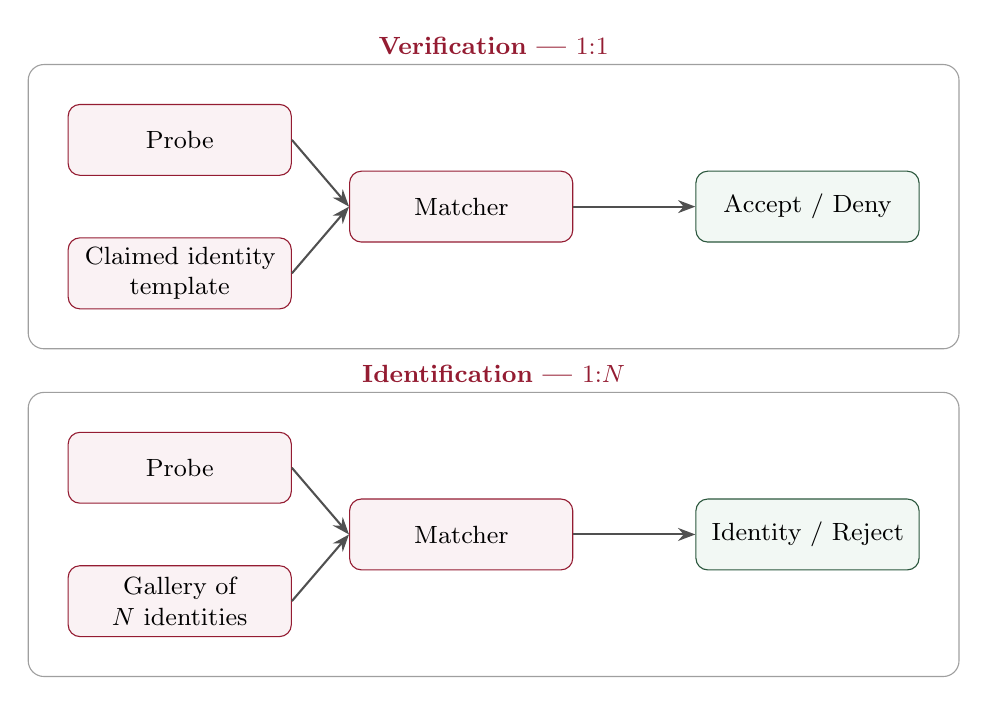
\begin{tikzpicture}[
    node distance=0.45cm,
%
    box/.style={
        draw=SapienzaRed,
        rounded corners=1.5mm,
        fill=SoftBlue,
        minimum width=2.8cm,
        text width=2.6cm,
        minimum height=0.9cm,
        align=center,
        font=\small
    },
%
    output/.style={
        draw=KeyGreen,
        rounded corners=1.5mm,
        fill=SoftGreen,
        minimum width=2.8cm,
        text width=2.6cm,
        minimum height=0.9cm,
        align=center,
        font=\small
    },
%
    arrow/.style={
        -{Stealth[length=2.2mm]},
        line width=0.75pt,
        color=MidGray
    },
%
    panel/.style={
        draw=MidGray!55,
        rounded corners=2mm,
        inner sep=5mm
    }
]
%
% Verification: the probe and the reference template are distinct matcher inputs.
%
\node[box] (vp) {Probe};
\node[
    box,
    below=0.78cm of vp
] (vclaim) {
    Claimed identity\\
    template
};
\node[
    box,
    right=2.15cm of $(vp)!0.5!(vclaim)$
] (vmatch) {Matcher};
\node[
    output,
    right=1.55cm of vmatch
] (vout) {Accept / Deny};
\draw[arrow] (vp.east) -- (vmatch.west);
\draw[arrow] (vclaim.east) -- (vmatch.west);
\draw[arrow] (vmatch) -- (vout);
\node[
    panel,
    fit=(vp)(vclaim)(vout),
    label={
        [font=\bfseries\small,text=SapienzaRed]
        above:Verification --- \(1{:}1\)
    }
] {};
%
% Identification: the probe and the gallery are distinct matcher inputs.
%
\node[
    box,
    below=3.25cm of vp
] (ip) {Probe};
\node[
    box,
    below=0.78cm of ip
] (igal) {
    Gallery of\\
    $N$ identities
};
\node[
    box,
    right=2.15cm of $(ip)!0.5!(igal)$
] (imatch) {Matcher};
\node[
    output,
    right=1.55cm of imatch
] (iout) {Identity / Reject};
\draw[arrow] (ip.east) -- (imatch.west);
\draw[arrow] (igal.east) -- (imatch.west);
\draw[arrow] (imatch) -- (iout);
\node[
    panel,
    fit=(ip)(igal)(iout),
    label={
        [font=\bfseries\small,text=SapienzaRed]
        above:Identification --- \(1{:}N\)
    }
] {};
%
\end{tikzpicture}

\else

\fbox{
\begin{minipage}{0.90\textwidth}

\textbf{Verification \(1{:}1\):}

Probe + claimed identity template
$\rightarrow$
Matcher
$\rightarrow$
Accept/Deny.

\textbf{Identification \(1{:}N\):}

Probe + gallery of \(N\) identities
$\rightarrow$
Matcher
$\rightarrow$
Identity/Reject.

\end{minipage}
}

\fi

\caption{
Verification compares a probe with a claimed identity,
whereas identification searches a gallery.
}
\label{fig:verification-identification}

\end{figure}

The structural difference between the two operations is summarized in
Figure~\ref{fig:verification-identification}.

\subsection{Open-set, Closed-set, and Lists}

In \emph{open-set identification}, the system determines whether a probe
\(p_i\) belongs to a subject represented in gallery \(G\).

Some probes may not correspond to any enrolled subject, so the system
needs a reject option.

Errors include rejecting an enrolled subject, accepting a non-enrolled
subject, or returning the wrong enrolled identity.

In \emph{closed-set identification}, all probes belong to enrolled
subjects.

The principal error is returning the wrong identity.

A \emph{watch list} contains subjects for whom the system checks
membership.

A \emph{white list} contains subjects who are granted access, whereas a
\emph{black list} contains subjects who are rejected or may trigger an
alarm.

\section{Requirements for a Biometric Trait}
\label{subsec:trait-requirements}

\begin{table}[htbp]
\centering
\caption{Requirements for a biometric trait.}
\label{tab:trait-requirements}
\small

\begin{tabular}{
    >{\bfseries}P{3.0cm}
    P{10.8cm}
}
\toprule

\rowcolor{SoftRed}
Requirement &
\textbf{Meaning}
\\

\midrule

Universality &
The trait should be possessed by every person, except for rare exceptions.
\\

Uniqueness &
Different people should be distinguishable according to the trait.
\\

Permanence &
The trait should remain sufficiently stable over time.
\\

Collectability &
The trait should be measurable by an appropriate sensor.
\\

Acceptability &
People should not object to collection or measurement of the trait.
\\

\bottomrule
\end{tabular}

\end{table}

The X9.84-2003 standard context includes fingerprints, iris and retina, face, ear, hand or finger geometry, signature, keystroke behaviour, voice, and DNA or other biological traces.

These modalities may be associated with physiological, behavioural,
or mixed features.

\section{Strong and Soft Biometric Traits}
\label{subsec:strong-soft}

Examples of \emph{strong biometric traits} include iris, face, and fingerprint, whereas \emph{soft biometric traits} include hair colour, facial shape, and gait.

Soft traits may lack uniqueness or long-term persistence; behavioural
characteristics can also be affected by transient conditions such as mood or
health. Even so, soft traits can reduce the search space by narrowing candidate
identities.


\section{Examples of Biometric Modalities}
\label{subsec:modalities}

A biometric modality determines both what is sensed and how the resulting
signal should be represented. Different modalities therefore require
different acquisition procedures, features, and matching strategies.

\subsection{Voice}

Voice recognition can represent speech through acoustic feature vectors.
A Gaussian Mixture Model (GMM) can model the distribution of those features:
training observations are collected for several acoustic dimensions, their
statistical distributions are estimated, and the resulting model is used to
score a new utterance. A representative score is a log-likelihood of the
form
\[
    \operatorname{score}
    =
    \log p(\text{speech}\mid\text{speaker model}).
\]
A larger likelihood indicates that the observed acoustic vectors are more
compatible with the stored model.

\subsection{Signature}

A signature may be treated as a static image or as a dynamic behavioural
signal. Dynamic acquisition can retain the trajectory of the pen together
with time-varying measurements. Representative features include the
\(x\)- and \(y\)-coordinates of the pen, pressure, pen azimuth in
\(0^\circ\)--\(359^\circ\), and pen altitude in \(0^\circ\)--\(90^\circ\).
The resulting template can therefore contain substantially more information
than the final ink trace alone.

\subsection{Fingerprint}

Fingerprint recognition uses information at different spatial levels.
First-level information captures global ridge-flow structure and broad
fingerprint patterns. Second-level information focuses on local minutiae,
such as ridge endings and bifurcations.

A typical processing chain begins from the fingerprint image, estimates the
orientation field, identifies a region of interest, extracts ridges, thins
the ridge representation, and finally extracts minutiae. Global ridge
patterns include arches, tented arches, loops, and whorls. Matching then
requires comparing the resulting local structures rather than merely
comparing two raw images pixel by pixel.

\subsection{Iris}

Iris recognition first captures an eye image and localizes the iris region.
One representative pipeline begins from a \(480\times640\) eye image. The
annular iris texture is then normalized or \emph{unwrapped}, encoded into a
compact feature representation, and compared with enrolled templates.
The comparison score is finally converted into an accept/reject decision.
This pipeline separates geometric normalization from texture encoding so that
matching can remain meaningful despite moderate changes in image scale or eye
position.

\subsection{Retina}

Retinal recognition is based on the vascular pattern visible on the
eyeground. The acquisition process captures the retina, localizes relevant
vascular structures, derives a representation of the vessel pattern, and
matches it against a stored template. The discriminative information is
therefore associated with the geometry of the capillary network rather than
with the external appearance of the eye.

\subsection{Face}

Face recognition admits several families of representations. Image-based
approaches include methods based on Independent Component Analysis (ICA),
neural networks, and eigenface-style representations. Feature-based
approaches can compare structured facial landmarks, for example through
elastic graph matching. Three-dimensional approaches can use 3D morphable
models, while hybrid approaches combine multiple descriptions such as
wavelet- or fractal-derived information.

\begin{table}[H]
\centering
\caption{Representative biometric modalities and the information used for matching.}
\label{tab:modalities}
\small
\begin{tabularx}{\textwidth}{
    >{\bfseries}P{2.4cm}
    P{5.1cm}
    X
}
\toprule
\rowcolor{SoftRed}
Modality & \textbf{Representative information} & \textbf{Typical comparison idea} \\
\midrule
Voice & Acoustic feature vectors and their statistical distribution &
Likelihood or vector-based comparison. \\
Signature & Static shape or dynamic pen trajectory, pressure, azimuth, altitude &
Image, sequence, or feature-vector matching. \\
Fingerprint & Global ridge flow and local minutiae &
Structured correspondence between ridge/minutia features. \\
Iris & Normalized iris texture encoding &
Template comparison after localization and normalization. \\
Retina & Vascular pattern on the eyeground &
Comparison of extracted vessel structures. \\
Face & Appearance, landmarks, learned features, or 3D structure &
Image-, feature-, embedding-, or model-based comparison. \\
\bottomrule
\end{tabularx}
\end{table}

\section{Benefits and Drawbacks of Biometric Traits}
\label{subsec:benefits-drawbacks}

Biometric traits provide a natural form of authentication because the user
need only appear in person.

They cannot be forgotten or lent in the same way as a password or token.

These advantages are accompanied by several drawbacks:

\begin{itemize}
    \item biometric systems do not provide \(100\%\) accuracy;

    \item some users cannot be reliably recognized by some technologies,
    for example when fingerprints are heavily worn or damaged;

    \item traits may change over time;

    \item biometric devices may be unreliable under some circumstances;

    \item a copied biometric trait cannot simply be replaced in the same
    way as a compromised password.
\end{itemize}

\begin{remarkbox}
A biometric characteristic is physically bound to the person, but a digital or physical representation of that characteristic can still be copied or compromised. Unlike a password, the underlying trait cannot simply be replaced after compromise.
\end{remarkbox}



\section{Chapter Summary}

Biometric systems treat personal identity as a pattern-recognition problem.
A complete system must acquire a suitable trait, extract a stable
representation, compare that representation with enrolled templates, and
convert the resulting score into a decision. Verification performs a
\(1{:}1\) comparison for a claimed identity, whereas identification searches
a \(1{:}N\) gallery and may additionally require a reject option. The
practical quality of a modality depends on universality, uniqueness,
permanence, collectability, and acceptability, while real deployments must
also account for acquisition conditions, user cooperation, imperfect
recognition, and the consequences of biometric compromise.

% ============================================================
\addtocontents{toc}{\protect\newpage}
\chapter[Performance Evaluation of Biometric Systems]{Performance Evaluation of \mbox{Biometric Systems}}
\label{sec:performance}

A biometric matcher does not return certainty; it returns evidence, usually
as a similarity or distance score. Performance evaluation studies how those
scores behave for genuine and impostor comparisons and how an operating
threshold converts them into correct decisions and errors.

% ============================================================

\section{Sources of Recognition Difficulty}
\label{subsec:difficulties}

Biometric recognition is difficult because the same person does not
always produce identical samples, while different people can sometimes
appear very similar according to the measured trait.

\begin{itemize}
    \item \textbf{Large intra-class variation}:
    samples from the same person may vary substantially,
    for example because of pose or facial expression.

    \item \textbf{Small inter-class variation}:
    samples from different people may be very similar,
    as illustrated by twins or close relatives.

    \item \textbf{Noisy or distorted acquisitions}:
    poor fingerprint quality or non-uniform illumination can degrade
    the sample.

    \item \textbf{Non-universality}:
    some people may not provide a usable sample for a particular modality.
    About \(4\%\) of the population is reported to present poor-quality
    fingerprints, with the issue being more frequent in some groups such as
    elderly people.

    \item \textbf{Spoofing and attacks}:
    attacks may target different points of the biometric processing
    pipeline.
\end{itemize}

Potential attack points span the complete biometric pipeline: the sensor, feature extractor, communication channels, matcher, stored templates, and final decision path.

Examples include presenting a fake biometric, replaying old data,
overriding feature extraction, synthesizing feature vectors, modifying
stored templates, overriding the matcher, intercepting channels, or
overriding the final decision.

\begin{keyconcept}
Performance is not determined only by the matcher.

It depends on acquisition quality, representation quality, population
variability, the operating threshold, and the integrity of the complete
biometric pipeline.
\end{keyconcept}

\section{Samples, Hand-crafted Features, and Templates}
\label{subsec:samples-features}

\begin{definitionbox}[ -- Sample]
A sample is the raw captured biometric data, such as an image,
a voice recording, or a fingerprint acquisition.
\end{definitionbox}

\begin{definitionbox}[ -- Hand-crafted Features]
Hand-crafted features are characteristics manually designed by a data
scientist and extracted from raw samples.
\end{definitionbox}

\begin{definitionbox}[ -- Template]
A template is a collection of features extracted from the raw biometric
data and used for comparison.
\end{definitionbox}

Templates may have different mathematical structures.

Representative template structures include:

\begin{itemize}
    \item a histogram of relevant image values such as grey levels;

    \item a vector of measurements, such as a collection of anthropometric
    measurements;

    \item a time series, such as acceleration values recorded along the
    three accelerometer axes;

    \item a set of fingerprint minutiae represented by triplets

    \[
        \set{
        (x_1,y_1,\theta_1),
        \ldots,
        (x_n,y_n,\theta_n)
        },
    \]

    where the coordinates identify relevant points and
    \(\theta_i\) represents the local ridge-tangent direction.
\end{itemize}

\section{Comparing Templates}
\label{subsec:template-comparison}

The comparison procedure depends on the representation.

Vector templates can often be compared with standard distances or
similarities, whereas structured representations may require specialized
matching.

\subsection{Euclidean Distance}

For vectors
\(
\mathbf{p},\mathbf{q}\in\R^n
\),
the Euclidean distance is
\begin{equation}
d(\mathbf{p},\mathbf{q})
=
\norm{\mathbf{p}-\mathbf{q}}_2
=
\sqrt{
\sum_{i=1}^{n}
(p_i-q_i)^2
}.
\label{eq:euclidean}
\end{equation}

Here \(n\) is the feature-space dimension, \(p_i\) and \(q_i\) are
corresponding vector components, and \(\lVert\cdot\rVert_2\) denotes the
Euclidean norm. A smaller Euclidean distance indicates greater similarity.

\subsection{Cosine Similarity}

The cosine similarity between vectors
\(
\mathbf{A}
\)
and
\(
\mathbf{B}
\)
is
\begin{equation}
S_C(\mathbf{A},\mathbf{B})
=
\cos(\theta)
=
\frac{
\mathbf{A}^{\mathsf T}\mathbf{B}
}{
\norm{\mathbf{A}}_2\,\norm{\mathbf{B}}_2
}
=
\frac{
\sum_{i=1}^{n} A_iB_i
}{
\sqrt{\sum_{i=1}^{n}A_i^2}\,
\sqrt{\sum_{i=1}^{n}B_i^2}
}.
\label{eq:cosine}
\end{equation}

Here \(\theta\) is the angle between the two vectors,
\(\mathbf{A}^{\mathsf T}\mathbf{B}\) is their dot product, and
\(\lVert\mathbf{A}\rVert_2\), \(\lVert\mathbf{B}\rVert_2\) are their
Euclidean norms. Unlike a distance, larger cosine similarity values represent
greater similarity.

\subsection{Pearson Correlation}

Pearson correlation can be used as a similarity measure for histograms
or sets of paired values.

Given paired samples
\(
(x_i,y_i)
\),
\(i=1,\ldots,n\),
\begin{equation}
r_{xy}
=
\frac{
\sum_{i=1}^{n}
(x_i-\bar{x})(y_i-\bar{y})
}{
\sqrt{
\sum_{i=1}^{n}(x_i-\bar{x})^2
}
\sqrt{
\sum_{i=1}^{n}(y_i-\bar{y})^2
}
}.
\label{eq:pearson-centered}
\end{equation}

An algebraically equivalent form is
\begin{equation}
r_{xy}
=
\frac{
n\sum_i x_i y_i
-
\left(\sum_i x_i\right)
\left(\sum_i y_i\right)
}{
\sqrt{
n\sum_i x_i^2
-
\left(\sum_i x_i\right)^2
}
\sqrt{
n\sum_i y_i^2
-
\left(\sum_i y_i\right)^2
}
}.
\label{eq:pearson-raw}
\end{equation}

Here \(\bar{x}\) and \(\bar{y}\) are the sample means and \(n\) is the
number of paired observations. The coefficient \(r_{xy}\) lies in the usual
correlation range and is interpreted here as a similarity measure.

\subsection{Bhattacharyya Distance}

For discrete probability distributions \(P\) and \(Q\) over the same
domain \(\mathcal{X}\), the Bhattacharyya coefficient is
\begin{equation}
BC(P,Q)
=
\sum_{x\in\mathcal{X}}
\sqrt{P(x)Q(x)}.
\label{eq:bhattacharyya-coeff}
\end{equation}

The corresponding distance is
\begin{equation}
D_B(P,Q)
=
-\ln\left(BC(P,Q)\right).
\label{eq:bhattacharyya}
\end{equation}

Here \(P(x)\) and \(Q(x)\) are the probability masses assigned to
\(x\in\mathcal{X}\), \(BC(P,Q)\) is the Bhattacharyya coefficient, and
\(D_B(P,Q)\) is the corresponding distance. This measure is useful for
comparing histogram-like or probabilistic representations.

\subsection{Dynamic Time Warping}

Dynamic Time Warping (DTW) is presented as a distance method for time
series.

The motivating example compares two repetitions of a walking sequence
recorded with motion capture.

Even when walking speeds differ, spatial trajectories may remain highly
similar.

DTW allows a non-linear alignment of time indices before comparison.

\subsection{Learned Features and Embeddings}

In deep-learning systems, the final classification layer, typically a softmax layer, can be omitted when the goal is to extract the internal \emph{embedding} that would otherwise feed the classifier.

These embeddings can then be treated as vectors and compared using
vector-based similarity or distance measures.

Some representations require more than direct vector comparison.

Fingerprint minutiae, for example, require finding a suitable pairing
between points before the match can be evaluated.

\begin{table}[htbp]
\centering
\caption{Comparison methods for representative biometric template structures.}
\label{tab:comparison-methods}
\small

\begin{tabular}{
    >{\bfseries}P{3.4cm}
    P{2.6cm}
    P{7.8cm}
}
\toprule

\rowcolor{SoftRed}
Method &
\textbf{Type} &
\textbf{Typical use}
\\

\midrule

Euclidean distance &
Distance &
Vector templates.
\\

Cosine similarity &
Similarity &
Vector templates and embeddings.
\\

Pearson correlation &
Similarity &
Histograms or paired point sets.
\\

Bhattacharyya distance &
Distance &
Histogram or distribution comparison.
\\

Dynamic Time Warping &
Distance &
Time-series comparison with temporal misalignment.
\\

Structured matching &
Task-specific &
Feature sets such as fingerprint minutiae where pairing is required.
\\

\bottomrule
\end{tabular}

\end{table}

\section{Similarity, Distance, and Acceptance Thresholds}
\label{subsec:thresholds}

Once a similarity or distance value has been obtained, it is compared
with an acceptance threshold in verification and open-set identification.

For a similarity score \(s\) and threshold \(t\),
\begin{equation}
\text{accept}
\quad\Longleftrightarrow\quad
s \geq t.
\label{eq:similarity-rule}
\end{equation}

For a distance \(d\),
\begin{equation}
\text{accept}
\quad\Longleftrightarrow\quad
d \leq t.
\label{eq:distance-rule}
\end{equation}

Reasoning with similarities and distances is symmetric after reversing
the inequality and the interpretation of larger and smaller values.

\section{Verification Outcomes}
\label{subsec:verification-outcomes}

A verification claim is accepted when the best matching score for the
claimed identity satisfies the threshold rule.

Four cases arise.

\begin{table}[htbp]
\centering
\caption{Verification outcomes and common biometric terminology.}
\label{tab:verification-outcomes}
\small

\begin{tabular}{
    P{3.0cm}
    P{2.55cm}
    P{4.15cm}
    P{4.15cm}
}
\toprule

\rowcolor{SoftRed}
\textbf{True situation} &
\textbf{System decision} &
\textbf{Biometric term} &
\textbf{Alternative term}
\\

\midrule

Genuine claim &
Accept &
Genuine Acceptance (GA) &
Genuine Match (GM)
\\

Genuine claim &
Reject &
False Rejection (FR) &
False Non-Match (FNM)
\\

Impostor claim &
Reject &
Genuine Rejection (GR) &
Genuine Non-Match (GNM)
\\

Impostor claim &
Accept &
False Acceptance (FA) &
False Match (FM)
\\

\bottomrule
\end{tabular}

\end{table}

\begin{remarkbox}[ -- Terminology note]
Type I and Type II depend on the choice of the null hypothesis.
With \(H_0=\text{different person}\), as defined below,
false acceptance is a Type I error and false rejection is a Type II error.
The opposite labels require \(H_0=\text{same person}\).

The biometric names FAR and FRR are the less ambiguous terms to use
when interpreting the hypothesis notation below.
\end{remarkbox}

\begin{remarkbox}[ -- Uncertain cases]
A practical possibility between automatic acceptance and rejection is to
route an uncertain score region to a human operator. Such a three-way policy is application-specific and does not change
the definitions of GA, GR, FA, and FR used for binary evaluation.
\end{remarkbox}

\section{False Acceptance Rate and False Rejection Rate}
\label{subsec:far-frr}

\noindent\begin{minipage}{\linewidth}
\setlength{\parskip}{0.50em}
\begin{metricbox}[ -- False Acceptance Rate (FAR/FMR)]
The False Acceptance Rate (FAR), also called False Match Rate (FMR), is
the fraction or probability of impostor recognition operations in which
the impostor is incorrectly accepted.
\end{metricbox}

For example,
\[
\mathrm{FAR}=0.1\%
\]
\nopagebreak
means that, on average, one out of every 1000 impostor attempts is
successful.
\end{minipage}\par

\noindent\begin{minipage}{\linewidth}
\setlength{\parskip}{0.50em}
\begin{metricbox}[ -- False Rejection Rate (FRR/FNMR)]
The False Rejection Rate (FRR), also called False Non-Match Rate (FNMR),
is the fraction or probability of genuine recognition operations in which
the genuine user is incorrectly rejected.
\end{metricbox}

For example,
\[
\mathrm{FRR}=0.05\%
\]
\nopagebreak
means that, on average, one out of every 2000 authorized access attempts
is incorrectly rejected.
\end{minipage}\par

\section{Ground Truth and Evaluation Notation}
\label{subsec:ground-truth}

Evaluation experiments use labelled samples, so the true identity is
known through a ground-truth function
\(
\id(\cdot)
\).

\begin{center}
\begin{tabularx}{\linewidth}{P{3.6cm} X}
\toprule
\rowcolor{SoftGray}
\textbf{Notation} & \textbf{Meaning} \\
\midrule
\(\id(p_j)\) & True identity of probe \(p_j\). \\
\(\id(g_x)\) & Identity associated with gallery template \(g_x\). \\
\(\topMatch(p_j,i)\) & Best match between probe \(p_j\) and the gallery template(s) associated with claimed identity \(i\). \\
\(s(t_1,t_2)\) & Matching score between two templates. \\
\bottomrule
\end{tabularx}
\end{center}

Let \(G=\{g_i\}\) denote the gallery templates. Let \(P_G\) be the set
of probes belonging to subjects represented in the gallery and \(P_N\) the
set of probes belonging to subjects not represented in the gallery.

For a genuine claim,
\begin{equation}
g_x
=
\topMatch\left(p_j,\id(p_j)\right),
\qquad
s_{xj}
=
s(g_x,p_j),
\qquad
p_j\in P_G.
\label{eq:genuine-topmatch}
\end{equation}

For an impostor claim,
\begin{equation}
g_x
=
\topMatch(p_j,i),
\qquad
i\neq\id(p_j),
\qquad
s_{xj}
=
s(g_x,p_j).
\label{eq:impostor-topmatch}
\end{equation}

Using the similarity-threshold convention,
\begin{equation}
\mathrm{FRR}(t)
=
\frac{
\abs{
\set{
p_j :
s_{xj}< t,
\;
\id(g_x)=\id(p_j)
}
}
}{
\abs{
\set{
p_j :
\id(g_x)=\id(p_j)
}
}
}.
\label{eq:frr}
\end{equation}

Similarly,
\begin{equation}
\mathrm{FAR}(t)
=
\frac{
\abs{
\set{
p_j :
s_{xj}\geq t,
\;
\id(g_x)\neq\id(p_j)
}
}
}{
\abs{
\set{
p_j :
\id(g_x)\neq\id(p_j)
}
}
}.
\label{eq:far}
\end{equation}

Two impostor scenarios are possible. An impostor may itself be registered but claim another identity, or may be completely outside the gallery.

For verification error computation, both are false claims.

\section{Genuine and Impostor Score Distributions}
\label{subsec:score-distributions}

A score is \emph{genuine} when it results from matching two samples from
the same enrolled individual.

A score is \emph{impostor} when it results from matching samples
associated with different identities.

The decision problem can be written through the hypotheses
\[
\begin{aligned}
H_0 &: \text{different person},\\
H_1 &: \text{same person}.
\end{aligned}
\]

Possible decisions are
\[
\begin{aligned}
D_0 &: \text{decide different person},\\
D_1 &: \text{decide same person}.
\end{aligned}
\]

The corresponding probabilities are
\begin{equation}
\mathrm{FAR}
=
\Prob(D_1\mid H_0),
\qquad
\mathrm{FRR}
=
\Prob(D_0\mid H_1).
\label{eq:hypothesis-errors}
\end{equation}

Figure~\ref{fig:score-distributions} gives a schematic view of the two
score distributions and the effect of a similarity threshold.

\begin{figure}[htbp]
\centering

\ifTikZAvailable

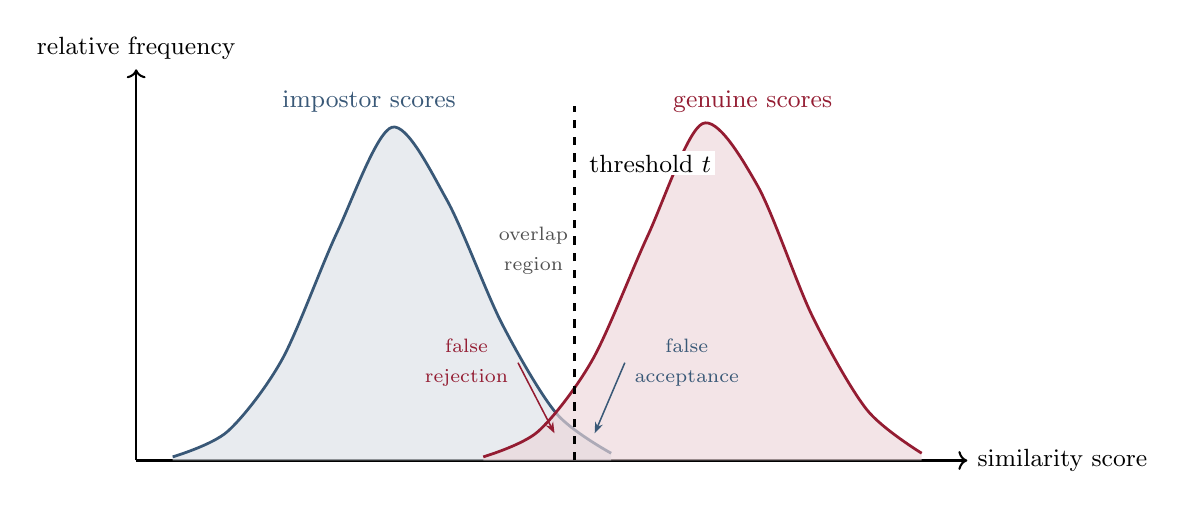
\begin{tikzpicture}[x=1.16cm,y=4.6cm]
%
    \draw[
        ->,
        line width=0.75pt
    ]
    (0,0)
    --
    (9.1,0)
    node[right]{\small similarity score};
%
    \draw[
        ->,
        line width=0.75pt
    ]
    (0,0)
    --
    (0,1.08)
    node[above]{\small relative frequency};
%
    % Impostor distribution
%
    \fill[
        PlotBlue!18,
        opacity=0.65
    ]
    plot[smooth] coordinates {
        (0.4,0.01)
        (1.0,0.08)
        (1.6,0.28)
        (2.2,0.63)
        (2.8,0.92)
        (3.4,0.72)
        (4.0,0.38)
        (4.6,0.13)
        (5.2,0.02)
    }
    --
    (5.2,0)
    --
    (0.4,0)
    --
    cycle;
%
    \draw[
        PlotBlue,
        line width=1.0pt,
        smooth
    ]
    plot coordinates {
        (0.4,0.01)
        (1.0,0.08)
        (1.6,0.28)
        (2.2,0.63)
        (2.8,0.92)
        (3.4,0.72)
        (4.0,0.38)
        (4.6,0.13)
        (5.2,0.02)
    };
%
    % Genuine distribution
%
    \fill[
        SapienzaRed!18,
        opacity=0.65
    ]
    plot[smooth] coordinates {
        (3.8,0.01)
        (4.4,0.08)
        (5.0,0.28)
        (5.6,0.62)
        (6.2,0.93)
        (6.8,0.76)
        (7.4,0.40)
        (8.0,0.14)
        (8.6,0.02)
    }
    --
    (8.6,0)
    --
    (3.8,0)
    --
    cycle;
%
    \draw[
        SapienzaRed,
        line width=1.0pt,
        smooth
    ]
    plot coordinates {
        (3.8,0.01)
        (4.4,0.08)
        (5.0,0.28)
        (5.6,0.62)
        (6.2,0.93)
        (6.8,0.76)
        (7.4,0.40)
        (8.0,0.14)
        (8.6,0.02)
    };
%
    % Threshold
%
    \draw[
        dashed,
        line width=0.85pt
    ]
    (4.8,0)
    --
    (4.8,0.98);
%
    \node[
        anchor=west,
        fill=white,
        inner sep=1.2pt
    ] at (4.92,0.82) {
        \small threshold \(t\)
    };
%
    \node[
        PlotBlue,
        fill=white,
        inner sep=1.1pt
    ]
    at (2.55,0.99) {
        \small impostor scores
    };
%
    \node[
        SapienzaRed,
        fill=white,
        inner sep=1.1pt
    ]
    at (6.75,0.99) {
        \small genuine scores
    };
%
    \node[
        align=center,
        PlotBlue,
        anchor=west
    ]
    (fa-label) at (5.35,0.27) {
        \scriptsize false\\[-0.1em]
        \scriptsize acceptance
    };
    \draw[
        -{Stealth[length=1.4mm]},
        PlotBlue,
        line width=0.55pt
    ] (fa-label.west) -- (5.02,0.075);
%
    \node[
        align=center,
        SapienzaRed,
        anchor=east
    ]
    (fr-label) at (4.18,0.27) {
        \scriptsize false\\[-0.1em]
        \scriptsize rejection
    };
    \draw[
        -{Stealth[length=1.4mm]},
        SapienzaRed,
        line width=0.55pt
    ] (fr-label.east) -- (4.58,0.075);
%
    \node[
        align=center,
        text=MidGray
    ]
    at (4.35,0.58) {
        \scriptsize overlap\\[-0.1em]
        \scriptsize region
    };
%
\end{tikzpicture}

\else

\fbox{
\begin{minipage}{0.88\textwidth}
\centering

Schematic score distributions:
impostor scores are concentrated toward lower similarity values,
genuine scores toward higher values, and a threshold in the overlap
region determines false acceptances and false rejections.

\end{minipage}
}

\fi

\caption{
Schematic genuine and impostor similarity-score distributions.
Numerical coordinates are used only to draw the conceptual shapes;
they do not represent experimental measurements.
}
\label{fig:score-distributions}

\end{figure}

\section{GAR, EER, ZeroFAR, and ZeroFRR}
\label{subsec:eer}

The Genuine Acceptance Rate (GAR), also called Genuine Match Rate (GMR),
is
\begin{equation}
\mathrm{GAR}
=
1-\mathrm{FRR}.
\label{eq:gar}
\end{equation}

The Equal Error Rate (EER) is the error level obtained at a threshold
\(t^\ast\) where
\begin{equation}
\mathrm{FAR}(t^\ast)
=
\mathrm{FRR}(t^\ast).
\label{eq:eer}
\end{equation}

Two limiting operating points are also useful:

\begin{itemize}
    \item \textbf{ZeroFRR / ZeroFNMR}:
    the FAR obtained when FRR is zero;

    \item \textbf{ZeroFAR / ZeroFMR}:
    the FRR obtained when FAR is zero.
\end{itemize}

For distance-based matching, an excessively low threshold produces many
genuine rejections, while an excessively high threshold produces many
false acceptances.

Under the similarity-threshold convention used in
Equations~\eqref{eq:similarity-rule},
\eqref{eq:frr},
and~\eqref{eq:far},
the direction is reversed:
increasing the threshold makes acceptance stricter,
so FAR decreases while FRR increases.

The EER threshold is a convenient and common comparison point because it
balances the two verification error rates. It is not automatically the best
operating threshold for a deployed application: the operating threshold must
follow the relative cost of false acceptances and false rejections.

Figure~\ref{fig:far-frr} shows the corresponding threshold trade-off
using the same similarity-threshold convention as
Equations~\eqref{eq:similarity-rule},
\eqref{eq:frr},
and~\eqref{eq:far}.

\begin{figure}[htbp]
\centering

\ifTikZAvailable

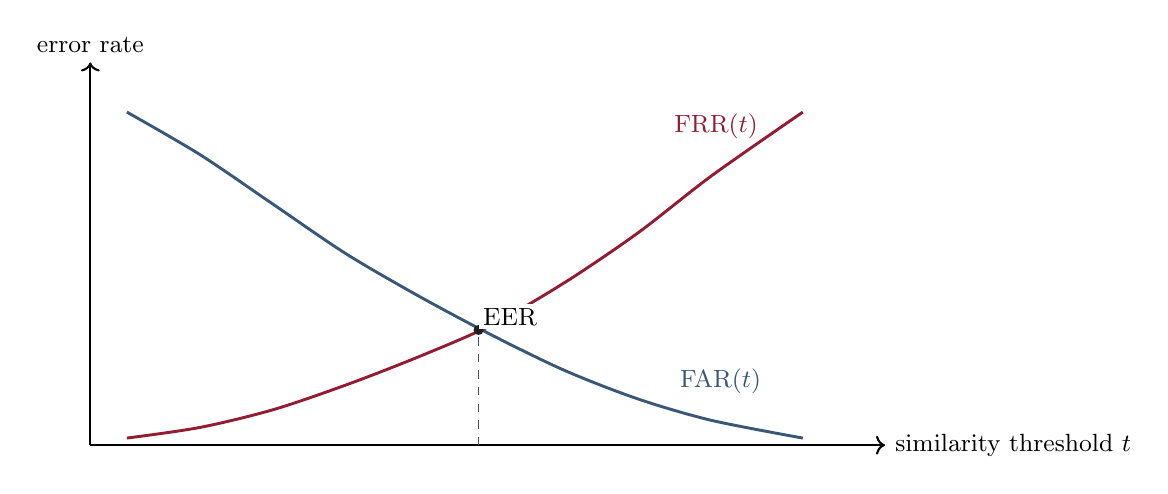
\begin{tikzpicture}[x=1.16cm,y=4.5cm]
%
    \draw[
        ->,
        line width=0.75pt
    ]
    (0,0)
    --
    (8.7,0)
    node[right]{
        \small similarity threshold \(t\)
    };
%
    \draw[
        ->,
        line width=0.75pt
    ]
    (0,0)
    --
    (0,1.08)
    node[above]{
        \small error rate
    };
%
    % FAR decreases as similarity threshold increases
%
    \draw[
        PlotBlue,
        line width=1.05pt,
        smooth
    ]
    plot coordinates {
        (0.4,0.94)
        (1.2,0.82)
        (2.0,0.68)
        (2.8,0.54)
        (3.6,0.42)
        (4.4,0.31)
        (5.2,0.21)
        (6.0,0.13)
        (6.8,0.07)
        (7.8,0.02)
    };
%
    % FRR increases as similarity threshold increases
%
    \draw[
        SapienzaRed,
        line width=1.05pt,
        smooth
    ]
    plot coordinates {
        (0.4,0.02)
        (1.2,0.05)
        (2.0,0.10)
        (2.8,0.17)
        (3.6,0.25)
        (4.4,0.34)
        (5.2,0.46)
        (6.0,0.60)
        (6.8,0.76)
        (7.8,0.94)
    };
%
    \fill[
        DarkText
    ]
    (4.25,0.325)
    circle
    (1.8pt);
%
    \draw[
        dashed,
        MidGray
    ]
    (4.25,0)
    --
    (4.25,0.325);
%
    \node[
        above right,
        fill=white,
        inner sep=1.5pt
    ]
    at (4.25,0.325) {
        \small EER
    };
%
    \node[
        PlotBlue
    ]
    at (6.9,0.18) {
        \small \(\mathrm{FAR}(t)\)
    };
%
    \node[
        SapienzaRed
    ]
    at (6.85,0.90) {
        \small \(\mathrm{FRR}(t)\)
    };
%
\end{tikzpicture}

\else

\fbox{
\begin{minipage}{0.88\textwidth}
\centering

For a similarity threshold, FAR decreases as the threshold increases,
whereas FRR increases.

Their intersection is the Equal Error Rate operating point.

\end{minipage}
}

\fi

\caption{
Schematic FAR/FRR trade-off under a
\emph{similarity-threshold} convention:
increasing \(t\) makes acceptance stricter,
so FAR decreases while FRR increases.
The intersection illustrates EER;
no experimental values are implied.
}
\label{fig:far-frr}

\end{figure}

\section{ROC and DET Curves}
\label{subsec:roc-det}

\begin{metricbox}[ -- ROC]
The Receiver Operating Characteristic (ROC) plots Genuine Acceptance Rate
\[
\mathrm{GAR}=1-\mathrm{FRR}
\]
\nopagebreak
against False Acceptance Rate (FAR) as the threshold varies.
\end{metricbox}

\begin{metricbox}[ -- DET]
The Detection Error Trade-off (DET) curve plots False Rejection Rate
(FRR) against False Acceptance Rate (FAR).

The standard DET uses normal-deviate (probit) axes:
the plotted coordinates are \(\Phi^{-1}(\mathrm{FAR})\) and
\(\Phi^{-1}(\mathrm{FRR})\), where \(\Phi\) is the standard normal CDF.
This is not a logarithmic scale.
\end{metricbox}

Each operating threshold corresponds to a point on the relevant
performance curve.

The two curve types are illustrated schematically in
Figures~\ref{fig:roc} and~\ref{fig:det}.

\begin{figure}[htbp]
\centering

\ifTikZAvailable

\begin{tikzpicture}[x=9.4cm,y=6.4cm]
%
    \draw[
        ->,
        line width=0.75pt
    ]
    (0,0)
    --
    (1.08,0)
    node[right]{
        \small FAR
    };
%
    \draw[
        ->,
        line width=0.75pt
    ]
    (0,0)
    --
    (0,1.08)
    node[above]{
        \small GAR
    };
%
    \draw[
        dashed,
        MidGray!70
    ]
    (0,0)
    --
    (1,1);
%
    \draw[
        SapienzaRed,
        line width=1.1pt,
        smooth
    ]
    plot coordinates {
        (0.00,0.00)
        (0.04,0.32)
        (0.10,0.54)
        (0.20,0.72)
        (0.35,0.84)
        (0.55,0.92)
        (0.75,0.97)
        (1.00,1.00)
    };
%
    \node[
        MidGray
    ]
    at (0.72,0.52) {
        \scriptsize reference diagonal
    };
%
\end{tikzpicture}

\else

\fbox{
\begin{minipage}{0.75\textwidth}
\centering

Schematic ROC:
GAR is plotted against FAR while the threshold varies.

\end{minipage}
}

\fi

\caption{
Schematic ROC representation with FAR on the horizontal axis
and GAR on the vertical axis.
The curve is illustrative only and contains no measured performance values.
}
\label{fig:roc}

\end{figure}

\begin{figure}[htbp]
\centering

\ifTikZAvailable

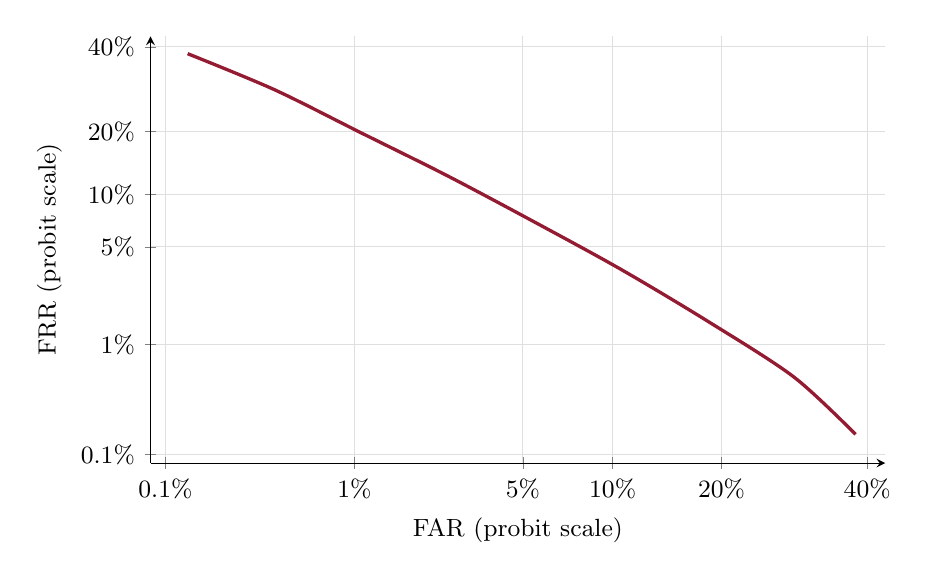
\begin{tikzpicture}
\begin{axis}[
    width=0.90\textwidth,
    height=7.0cm,
    xmin=-3.15,
    xmax=-0.18,
    ymin=-3.15,
    ymax=-0.18,
    axis lines=left,
    xlabel={FAR (probit scale)},
    ylabel={FRR (probit scale)},
    xtick={-3.090,-2.326,-1.645,-1.282,-0.842,-0.253},
    ytick={-3.090,-2.326,-1.645,-1.282,-0.842,-0.253},
    xticklabels={0.1\%,1\%,5\%,10\%,20\%,40\%},
    yticklabels={0.1\%,1\%,5\%,10\%,20\%,40\%},
    tick label style={font=\small},
    label style={font=\small},
    grid=major,
    grid style={draw=MidGray!18},
    clip=false
]
\addplot[
    SapienzaRed,
    very thick,
    smooth
] coordinates {
    (-3.00,-0.30)
    (-2.65,-0.55)
    (-2.30,-0.85)
    (-1.95,-1.15)
    (-1.60,-1.47)
    (-1.25,-1.80)
    (-0.90,-2.16)
    (-0.55,-2.55)
    (-0.30,-2.95)
};
\end{axis}
\end{tikzpicture}

\else

\fbox{
\begin{minipage}{0.78\textwidth}
\centering

Schematic DET on normal-deviate axes:
the coordinates are \(\Phi^{-1}(\mathrm{FAR})\) and
\(\Phi^{-1}(\mathrm{FRR})\).

\end{minipage}
}

\fi

\caption{
Schematic DET representation. Both axes are normal-deviate (probit)
transforms of the corresponding error probabilities; the tick labels show
the original FAR and FRR percentages. The curve is conceptual and does not
encode experimental measurements.
}
\label{fig:det}

\end{figure}

\begin{keyconcept}
For ROC curves, better systems tend toward high GAR at low FAR, i.e. toward
the upper-left operating region. For DET curves, better systems tend toward
simultaneously low FAR and low FRR, i.e. toward the lower-left region. Curve
comparisons must still be made at operating points relevant to the intended
application.
\end{keyconcept}

\section{Open-set Identification Performance}
\label{subsec:open-set-performance}

In open-set identification, such as a watch-list application,
the system addresses two questions:

\begin{enumerate}
    \item Is the probe subject represented in the gallery?

    \item If so, who is the probe subject?
\end{enumerate}

Open-set identification combines ranked similarity scores with an acceptance threshold.

For a probe belonging to a gallery subject, correct operation requires
both detection above the threshold and correct ranking of the true
identity.

For a probe outside the gallery, correct operation requires that no
gallery candidate incorrectly triggers an alarm.

Typical open-set applications include comparing people observed in an airport
against a watch list or comparing an unidentified person against a missing-person
database. These applications require both a membership decision and, when a
match is detected, an identity decision.

\begin{examplebox}[ -- Thresholded ranked scores]

Suppose four candidates obtain scores
\[
0.90,\;0.86,\;0.60,\;0.40.
\]

With a similarity threshold of \(0.85\),
two candidates exceed the threshold.

If the top-ranked candidate is the correct identity,
the operation is both a correct detection and a correct identification.

Raising the threshold to \(0.95\) produces no detection.

If the correct identity is not the highest-scoring candidate,
detection can occur without correct identification. For example, with scores
\(0.86,0.80,0.60,0.40\) and threshold \(0.75\), detection occurs, but the
operation is not a correct detect-and-identify if the true identity is the
second-ranked candidate.

For a probe from outside the gallery, scores
\(0.80,0.70,0.60,0.40\) with threshold \(0.85\) produce no alarm and
therefore a correct rejection. Lowering the threshold to \(0.75\) makes the
highest score trigger an alarm, which is a false alarm because the probe has
no mated gallery identity.

\end{examplebox}

For probes from \(P_G\), repeated trials estimate how often the system
correctly detects and identifies the subject.

This quantity is the \emph{correct detect and identify rate}.

For probes from \(P_N\), repeated trials estimate how often an incorrect
alarm occurs.

This is the \emph{false alarm rate}.

\subsection{Rank and DIR}

Let \(\rankop(p_j)\) denote the position in the ranked list at which the first template for
the correct identity appears.

The Detection and Identification Rate, \(\mathrm{DIR}(t,k)\), expresses the
probability that a gallery probe is detected above operating threshold \(t\)
and that the correct identity appears within the first \(k\) ranked candidates.
For similarity scores, a precise form is
\begin{equation}
\mathrm{DIR}(t,k)
=
\frac{
\left|
\left\{
 p_j\in P_G:
 \rankop(p_j)\le k,
 \max_{g_i\in G:\,\id(g_i)=\id(p_j)} s(g_i,p_j)\ge t
\right\}
\right|
}{|P_G|}.
\label{eq:dir}
\end{equation}
Here \(k\) is the maximum accepted rank, \(t\) is the similarity threshold,
and the inner maximum selects the best mated gallery template for probe \(p_j\).

At rank 1, the corresponding False Negative Identification Rate (FNIR) is
\begin{equation}
\mathrm{FNIR}(t)
=
1-\mathrm{DIR}(t,1).
\label{eq:fnir}
\end{equation}
The explicit threshold dependence is important in open-set evaluation because
changing \(t\) changes both the detection probability and the false-alarm rate.

The false-alarm counterpart is the False Positive Identification Rate
(FPIR), also described as FAR or false alarm rate in a watch-list context. For
non-enrolled probes,
\begin{equation}
\mathrm{FPIR}(t)
=
\frac{
\left|
\left\{
 p_j\in P_N:
 \max_{g_i\in G}s(g_i,p_j)\ge t
\right\}
\right|
}{|P_N|}.
\label{eq:fpir}
\end{equation}
Thus \(G\) is the gallery, \(P_N\) is the set of non-gallery probes, and an
alarm occurs whenever at least one gallery score reaches the similarity
threshold. The same quantity is also described using FAR/false-alarm terminology in some
contexts; FPIR is the more task-specific name in open-set identification.

At rank 1, an open-set equal-error operating point can be described by
\(\mathrm{FNIR}(t)=\mathrm{FPIR}(t)\), i.e. by equalizing the paired
open-set error probabilities.

\subsection{Open-set ROC and Operating Regions}

The detect-and-identify rate and false-alarm rate vary in opposite
directions with the threshold.

Raising a similarity threshold tends to reduce both successful detection
and false alarms.

Lowering the threshold tends to increase both.

Five practical operating preferences can be distinguished:

\begin{enumerate}
    \item extremely low false alarm;

    \item extremely high detection and identification probability;

    \item low false alarm with lower detection and identification;

    \item high detection and identification with higher false alarms;

    \item no fixed threshold, with ranked results returned for
    investigation.
\end{enumerate}

\section{Closed-set Identification Performance}
\label{subsec:closed-set-performance}

Closed-set identification is a special case in which every probe is
known to have a corresponding identity in the gallery.

The membership question is therefore already answered.

Pure closed-set operation is relatively restrictive in practice. A system may
be described broadly as an identification system while operationally behaving
like a watch list; the FBI Integrated Automated Fingerprint Identification
System (IAFIS) is a representative example of this distinction.

The remaining issue is how highly the correct identity is ranked.

If the correct identity has the highest similarity score,
the system has achieved correct identification at rank 1.

If the correct identity has the second-highest score,
it is within the top two results and contributes to correct
identification at rank 2.

\Needspace{5cm}
\begin{examplebox}[ -- Closed-set ranks]
With similarity scores \(0.90,0.86,0.60,0.40\), a correct identity in the
first position gives a rank-1 identification. With scores
\(0.86,0.80,0.60,0.40\), if the correct identity is the second-ranked
candidate, the result contributes to identification at rank 2 even though it
is not correct at rank 1. More generally, rank \(k\) asks whether the correct
identity appears anywhere within the first \(k\) candidates.
\end{examplebox}

\begin{metricbox}[ -- Cumulative Match Score (CMS)]
The CMS at rank \(k\) is the probability that the correct identity is
found among the first \(k\) positions of the ranked candidate list.

Equivalently, it can be estimated as the fraction of test probes whose
correct identity appears within the top \(k\) results.
\end{metricbox}

\begin{metricbox}[ -- Cumulative Match Characteristic (CMC)]
A CMC curve plots the cumulative match score as a function of rank.

CMS at rank 1 gives the probability that the correct identity is the
first returned candidate.

CMS at rank 2 gives the probability that it appears in either of the
first two positions.

More generally, CMS at rank \(k\) gives the probability that the correct
identity appears among the first \(k\) positions.
\end{metricbox}

When the rank reaches the gallery size,
the cumulative probability reaches 1 because the correct identity must
occur somewhere in the complete closed-set list.

CMS at rank 1 is also called the \emph{Recognition Rate (RR)}.

Figure~\ref{fig:cmc} visualizes this cumulative ranking behaviour.

\begin{figure}[htbp]
\centering

\ifTikZAvailable

\begin{tikzpicture}[x=1.08cm,y=5.5cm]
%
    \draw[
        ->,
        line width=0.75pt
    ]
    (0,0)
    --
    (10.0,0)
    node[right]{
        \small rank \(k\)
    };
%
    \draw[
        ->,
        line width=0.75pt
    ]
    (0,0)
    --
    (0,1.08)
    node[above]{
        \small CMS
    };
%
    \draw[
        SapienzaRed,
        line width=1.1pt
    ]
    plot[smooth] coordinates {
        (1,0.48)
        (2,0.63)
        (3,0.73)
        (4,0.81)
        (5,0.87)
        (6,0.91)
        (7,0.95)
        (8,0.975)
        (9,0.99)
    };
%
    \foreach \x in {1,...,9}{
        \draw
        (\x,0.012)
        --
        (\x,-0.012)
        node[below=2pt]{
            \scriptsize \x
        };
    }
%
    \fill[
        SapienzaRed
    ]
    (1,0.48)
    circle
    (1.7pt);
%
    \node[
        above right
    ]
    at (1,0.48) {
        \small RR = CMS@1
    };
%
\end{tikzpicture}

\else

\fbox{
\begin{minipage}{0.80\textwidth}
\centering

A CMC curve is non-decreasing with rank.

CMS at rank 1 is the Recognition Rate,
and the cumulative probability approaches 1 as the complete closed-set
candidate list is included.

\end{minipage}
}

\fi

\caption{
Schematic cumulative match characteristic (CMC)
for closed-set identification.
The curve illustrates cumulative ranking behaviour only;
no dataset-specific values are implied.
}
\label{fig:cmc}

\end{figure}

\Needspace{6cm}
\section{Avoiding Confusion with Machine-Learning Metrics}
\label{subsec:ml-confusion}

Biometric error measures should not be confused with precision, recall, and F-score.

In standard machine-learning notation, let \(TP\), \(FP\), \(TN\), and
\(FN\) denote true positives, false positives, true negatives, and false
negatives, respectively. Then
\begin{equation}
\mathrm{Precision}
=
\frac{TP}{TP+FP},
\qquad
\mathrm{Recall}
=
\frac{TP}{TP+FN}.
\label{eq:precision-recall}
\end{equation}
The F-score combines precision and recall; it is therefore also conceptually
different from FAR and FRR.

In biometric acceptance/rejection terms,
precision can be compared with
\[
\frac{GA}{FA+GA},
\]
\nopagebreak
while recall can be compared with
\[
\frac{GA}{GA+FR}.
\]

The biometric error rates of primary interest are instead
\begin{equation}
\mathrm{FRR}
=
\frac{FR}{GA+FR},
\qquad
\mathrm{FAR}
=
\frac{FA}{FA+GR}.
\label{eq:biometric-error-counts}
\end{equation}

Under the mapping
acceptance
\(
\leftrightarrow
\)
positive
and rejection
\(
\leftrightarrow
\)
negative,
\begin{equation}
\mathrm{FRR}
=
\frac{FN}{TP+FN},
\qquad
\mathrm{FAR}
=
\frac{FP}{FP+TN}.
\label{eq:ml-mapping}
\end{equation}

Thus FRR corresponds to the false-negative rate or miss rate,
while FAR corresponds to the false-positive rate or fall-out.

Precision and recall therefore do not express the same error statistics
as FAR and FRR.

\Needspace{0.52\textheight}
\section{Identification versus Re-identification}
\label{subsec:reid}

Biometric identification and re-identification (re-ID) address related but different tasks.

\begin{table}[htbp]
\centering
\caption{Identification and re-identification as related recognition tasks.}
\label{tab:identification-reid}
\small

\begin{tabular}{
    >{\bfseries}P{3.0cm}
    P{6.2cm}
    P{4.8cm}
}
\toprule

\rowcolor{SoftRed}
Task &
\textbf{Objective} &
\textbf{Time perspective / context}
\\

\midrule

Identification &
Determine the identity of an unknown subject. &
Medium-to-long-term identity recognition.
\\

Re-identification &
Match the presence of the same person across different cameras,
locations, video segments, image sequences, or event sets using appearance,
body shape, behaviour, and tracking information. &
Short-term association across non-overlapping time slices.
\\

\bottomrule
\end{tabular}

\end{table}

Re-identification is evaluated with metrics adapted to ranked retrieval.

CMC is appropriate when there is a single mated gallery image for each
query.

When several mated images may exist,
Average Precision (AP) and mean Average Precision (mAP) are used.

AP is described as the area under a precision--recall curve computed
over thresholds, while mAP averages AP over queries.

Re-identification can connect back to identification when a person is
repeatedly found in video and the resulting identity evidence is then
checked against a watch list.

% ============================================================
\section{Chapter Summary}
\label{sec:performance-summary}

Performance evaluation connects matcher scores to operational error probabilities. The principal measures for verification and identification are consolidated below.

% ============================================================

\begin{table}[htbp]
\centering
\caption{Compact summary of central biometric performance measures.}
\label{tab:summary-metrics}
\small

\begin{tabular}{
    >{\bfseries}P{2.3cm}
    P{3.7cm}
    P{7.9cm}
}
\toprule

\rowcolor{SoftRed}
Measure &
\textbf{Main task} &
\textbf{Meaning}
\\

\midrule

FAR / FMR &
Verification &
Probability or fraction of impostor claims incorrectly accepted.
\\

FRR / FNMR &
Verification &
Probability or fraction of genuine claims incorrectly rejected.
\\

GAR / GMR &
Verification &
Genuine acceptance probability;
\(1-\mathrm{FRR}\).
\\

EER &
Verification / open set &
Operating point where paired error rates are equal.
\\

DIR &
Open-set identification &
Detection and identification performance at a chosen rank.
\\

FNIR &
Open-set identification &
False negative identification rate.
\\

FPIR &
Open-set identification &
False positive identification or false alarm probability.
\\

CMS@\(k\) &
Closed-set identification &
Probability that the correct identity appears among the first \(k\)
ranked candidates.
\\

CMC &
Closed-set identification &
Curve of CMS values across ranks.
\\

RR &
Closed-set identification &
Recognition rate, equal to CMS at rank 1.
\\

\bottomrule
\end{tabular}

\end{table}

% ============================================================
\clearpage
\renewcommand{\bibname}{References}
\gdef\CurrentSectionMark{}
\markboth{References}{References}
% ============================================================

\begingroup
\normalsize
\begin{thebibliography}{99}
\setlength{\itemsep}{0.65em plus 0.1em}
\setlength{\parsep}{0pt}
\raggedright
\addcontentsline{toc}{chapter}{References}

\bibitem{jain-handbook}
A. K. Jain, P. Flynn, and A. A. Ross,
\emph{Handbook of Biometrics}. Springer, 2008.

\bibitem{wechsler-face}
H. Wechsler,
\emph{Reliable Face Recognition Methods: System Design, Implementation and Evaluation}.
Springer, 2007.

\bibitem{ross-multibiometrics}
A. Ross, K. Nandakumar, and A. K. Jain,
\emph{Handbook of Multibiometrics}. Springer, 2006.

\bibitem{drygajlo-2007}
A. Drygajlo, \emph{Biometrics for Identity Verification}, 2007.

\bibitem{daugman-patent}
J. Daugman, ``Biometric Personal Identification System Based on Iris Analysis,''
U.S. Patent 5,291,560, 1994.

\bibitem{nappi-2009}
M. Nappi, \emph{Sistemi Biometrici}, 2009.

\bibitem{riccio-2007}
D. Riccio, \emph{Face Recognition}, 2007.

\bibitem{bolle-roc-cmc}
R. M. Bolle, J. H. Connell, S. Pankanti, N. K. Ratha, and A. W. Senior,
``The Relation between the ROC Curve and the CMC,'' Fourth IEEE Workshop on
Automatic Identification Advanced Technologies (AutoID'05), pp. 15--20, 2005.

\bibitem{doddington-menagerie}
G. Doddington, W. Liggett, A. Martin, M. Przybocki, and D. Reynolds,
``Sheeps, goats, lambs and wolves: A statistical analysis of speaker performance
in the NIST 1998 speaker recognition evaluation,'' Proc. ICSLD, 1998.

\bibitem{teli-zoos}
M. N. Teli, J. R. Beveridge, P. J. Phillips, G. H. Givens, D. S. Bolme,
and B. A. Draper, ``Biometric Zoos: Theory and Experimental Evidence.''

\bibitem{yager-menagerie}
N. Yager and T. Dunstone,
``Worms, Chameleons, Phantoms and Doves: New Additions to the Biometric
Menagerie,'' IEEE Workshop on Automatic Identification Advanced Technologies,
pp. 1--6, 2007.

\bibitem{torralba-dataset-bias}
A. Torralba and A. A. Efros,
``Unbiased look at dataset bias,'' IEEE Conference on Computer Vision and
Pattern Recognition (CVPR), pp. 1521--1528, 2011.

\bibitem{kryszczuk-fusion}
K. Kryszczuk, J. Richiardi, P. Prodanov, and A. Drygajlo,
``Reliability-based decision fusion in multimodal biometric verification,''
EURASIP Journal on Advances in Signal Processing, Article ID 86572, 2007.

\bibitem{demarsico-quality}
M. De Marsico, M. Nappi, and D. Riccio,
``Measuring measures for face sample quality,'' Proc. 3rd International ACM
Workshop on Multimedia in Forensics and Intelligence, pp. 7--12, 2011.

\bibitem{poh-fusion}
N. Poh and S. Bengio,
``Improving Fusion with Margin-Derived Confidence in Biometric Authentication
Tasks,'' IDIAP-RR 04-63, 2004.

\bibitem{demarsico-nabs}
M. De Marsico, M. Nappi, D. Riccio, and G. Tortora,
``NABS: Novel Approaches for Biometric Systems,'' IEEE Transactions on Systems,
Man, and Cybernetics -- Part C: Applications and Reviews, vol. 41, no. 4,
pp. 481--493, 2011.

\end{thebibliography}
\endgroup

% ============================================================
\chapter*{Quick Review}
\addcontentsline{toc}{chapter}{Quick Review}
\gdef\CurrentSectionMark{}
\markboth{Quick Review}{Quick Review}
% ============================================================

The most exam-relevant relationships are grouped below for rapid review.

\begingroup
\normalsize
\raggedright
\tcbset{before skip=8pt,after skip=8pt,before upper=\raggedright}
\noindent\begin{minipage}[t]{0.485\textwidth}
\vspace{0pt}
\begin{keyconcept}
\textbf{Foundations and architecture}
\begin{itemize}[leftmargin=*,itemsep=0.18em,topsep=0.25em]
    \item Biometrics is pattern recognition in which the classes are individual people.
    \item A biometric system uses acquisition, feature extraction, matching, and decision modules.
    \item Enrollment creates reference templates; recognition compares a probe with stored templates.
    \item Verification is \(1{:}1\); identification is \(1{:}N\).
    \item A useful trait should provide universality, uniqueness, permanence, collectability, and acceptability.
    \item Controlled acquisition reduces nuisance variation; uncontrolled acquisition may not permit recapture.
\end{itemize}
\end{keyconcept}

\begin{remarkbox}[ -- Matching rules]
\[
\begin{aligned}
\text{similarity: accept} &\iff s\ge t,\\
\text{distance: accept} &\iff d\le t.
\end{aligned}
\]
Increasing a \emph{similarity} threshold makes acceptance stricter; increasing a
\emph{distance} threshold makes acceptance looser.
\end{remarkbox}

\end{minipage}\hfill
\begin{minipage}[t]{0.485\textwidth}
\vspace{0pt}
\begin{metricbox}[ -- Verification]
\begin{itemize}[leftmargin=*,itemsep=0.18em,topsep=0.25em]
    \item FAR/FMR: impostor claim incorrectly accepted.
    \item FRR/FNMR: genuine claim incorrectly rejected.
    \item GAR/GMR: \(1-\mathrm{FRR}\).
    \item EER: operating point where FAR and FRR are equal.
    \item Genuine and impostor score distributions overlap; the threshold divides that overlap into false acceptances and false rejections.
    \item ROC plots GAR versus FAR. DET plots FRR versus FAR on normal-deviate (probit) axes.
\end{itemize}
\end{metricbox}


\begin{metricbox}[ -- Identification]
\begin{itemize}[leftmargin=*,itemsep=0.18em,topsep=0.25em]
    \item Open set asks both whether the probe belongs to the gallery and, if so, who it is.
    \item DIR\((t,k)\): successful detection with the correct identity within the first \(k\) ranks.
    \item FNIR\((t)=1-\mathrm{DIR}(t,1)\).
    \item FPIR: false alarm probability for non-gallery probes.
    \item Closed set assumes every probe has a gallery mate and is evaluated by rank.
    \item CMS@\(k\): probability that the correct identity is within the first \(k\) candidates.
    \item CMC plots CMS versus rank; CMS@1 is the Recognition Rate.
\end{itemize}
\end{metricbox}

\end{minipage}\par
\endgroup
\clearpage
\begingroup
\tcbset{before upper=\raggedright}
\noindent\begin{minipage}[t]{0.485\textwidth}
\vspace{0pt}
\raggedright
\begin{remarkbox}[ -- Do not confuse]
\begin{itemize}[leftmargin=*,itemsep=0.18em,topsep=0.25em]
    \item FAR and FRR are not precision and recall. FAR corresponds to FPR/fall-out; FRR corresponds to FNR/miss rate.
    \item Type I/II labels depend on the null hypothesis. FAR/FRR terminology is safer.
    \item Standard DET axes are probit, not ordinary logarithmic axes.
    \item EER is a comparison point, not a universally optimal deployment threshold.
    \item A raw sample is distinct from the feature representation or template extracted from it.
\end{itemize}
\end{remarkbox}

\end{minipage}\hfill
\begin{minipage}[t]{0.485\textwidth}
\vspace{0pt}
\raggedright
\begin{keyconcept}
\textbf{Modalities and representations}
\begin{itemize}[leftmargin=*,itemsep=0.18em,topsep=0.25em]
    \item Strong biometric traits aim at identity discrimination; soft traits mainly narrow the candidate set.
    \item Vector templates may use Euclidean distance or cosine similarity; histograms/\allowbreak distributions may use correlation or Bhattacharyya distance; time series may use DTW.
    \item Learned embeddings can be compared as vectors; structured templates such as fingerprint minutiae require task-specific correspondence.
    \item Re-identification is ranked retrieval across observations: CMC is useful for a single mated gallery image, while AP/mAP address multiple relevant matches.
\end{itemize}
\end{keyconcept}
\end{minipage}\par

\begin{remarkbox}[ -- Compact equation sheet]
\small
\begin{tabularx}{\linewidth}{>{\bfseries}P{3.0cm} X}
Verification &
\(\displaystyle \mathrm{FAR}=\frac{FA}{FA+GR}\),\quad
\(\displaystyle \mathrm{FRR}=\frac{FR}{GA+FR}\),\quad
\(\mathrm{GAR}=1-\mathrm{FRR}\). \\
\addlinespace[2pt]
Equal error &
\(\mathrm{FAR}(t^\ast)=\mathrm{FRR}(t^\ast)\). \\
\addlinespace[2pt]
Open set &
\(\mathrm{FNIR}(t)=1-\mathrm{DIR}(t,1)\); FPIR is the fraction of non-gallery probes whose best gallery score reaches the threshold. \\
\addlinespace[2pt]
Closed set &
\(\mathrm{RR}=\mathrm{CMS}@1\); \(\mathrm{CMS}@k\) is the probability that the correct identity is within the first \(k\) candidates. \\
\end{tabularx}
\normalsize
\end{remarkbox}

\endgroup
\end{document}
